\documentclass[14pt,a4paper]{extarticle}
%\documentclass[12pt,a4paper]{article}

\usepackage[utf8]{inputenc}
\usepackage[ukrainian]{babel}


\usepackage{amssymb}
\usepackage{physics}


\usepackage[active]{srcltx}
\usepackage[final]{pdfpages}

\usepackage[hidelinks]{hyperref}

\usepackage{verbatim}
%%%%%%%%%%%%%%%%%%%%%%%%%%%%%%%%%%%%%%%%%%%%%%%%%%%%%%%%%%%%%%%%%%
%\pagestyle{empty}                     %нумерацiя сторiнок i т.д.
\pagestyle{headings}                   %нумерацiя сторiнок вгорi зправа i т.д.
%\renewcommand{\baselinestretch}{1.5}   %мiжстрiчковий інтервал
%\parindent=7.5mm                      %абзацний відступ
 \righthyphenmin=2                     %перенос 2 останніх букв
 \pagenumbering{arabic}
 \tolerance=400
 \mathsurround=2pt
 \hfuzz=1.5pt
%%%%%%%%%%%%%%%%%%%%%%%%%%%%%%%%%%%%%%%%%%%%%%%%%%%%%%%%%%%%%%%%%%
 \hoffset=-0.5cm        %+2.5cm -- вiдступ вiд лiвого краю
 \voffset=-1.5cm        %+2.5cm -- вiдступ зверху
 \oddsidemargin=0.1cm   %ліве поле
 \topmargin=0.1cm       %верхнє поле
 \headheight=0.5cm      %висота верхнього колонтитулу
 \footskip=1cm          %висота нижнього колонтитулу
 \headsep=0.3cm         %відступ від колонт. до тексту
 \textwidth=17cm        %ширина сторінки
 \textheight=25.5cm     %висота сторінки
%%%%%%%%%%%%%%%%%%%%%%%%%%%%%%%%%%%%%%%%%%%%%%%%%%%%%%%%%%%%%%%%%%
 \newcounter{e}
 \setcounter{e}{0}
 \newcommand{\n}{\refstepcounter{e} (\arabic{e})}
 
 \newcounter{pic}
 \setcounter{pic}{0}
 \newcommand{\pic}[1]{\refstepcounter{pic} \vspace{-0.3cm}\textit{Рисунок \arabic{pic}\label{#1}.}}
 
 \newcounter{tabl}
 \setcounter{tabl}{0}
 \newcommand{\tabl}[1]{\refstepcounter{tabl} \vspace{-0.3cm}\textit{Таблиця \arabic{tabl}\label{#1}.}}
 
 \newcounter{dod}
 \setcounter{dod}{0}
 \newcommand{\dod}[1]{\refstepcounter{dod} \textit{Додаток \arabic{dod}\label{#1}.}}
 
 \newcounter{defn}
 \setcounter{defn}{0}
 \newcommand{\defn}[1]{\refstepcounter{defn} \textbf{Означення \arabic{defn}\label{#1}.}}
 
 \newcounter{theorem}
 \setcounter{theorem}{0}
 \newcommand{\theorem}[1]{\refstepcounter{theorem} \textbf{Теорема \arabic{theorem}\label{#1}.}}
 
 \newcommand{\proof}{\textit{Доведення. \space}}
% \setcounter{page}{1}
% \setcounter{section}{1}
%%%%%%%%%%%%%%%%%%%%%%%%%%%%%%%%%%%%%%%%%%%%%%%%%%%%%%%%%%%%%%%%%%
 \newcounter{stali}
 \setcounter{stali}{0}
 \newcommand{\s}{\refstepcounter{stali} \arabic{stali}}

 \newcommand{\st}{C_{\s}}
 \newcommand{\stl}[1]{C_{\s \label{#1}}}

 \newcommand{\cd}{{} $$ \vspace{-0.3cm} $$ {}}
 
 \newcommand{\nb}[2]{\righthyphenmin=#2 #1 \righthyphenmin=2}

%%%%%%%%%%%%%%%%%%%%%%%%%%%%%%%%%%%%%%%%%%%%%%%%%%%%%%%%%%%%%%%%%%
 
 \newcommand{\tabboxl}[2]{\parbox{#1}{\vspace{0.1cm} #2 \vspace{0.1cm} }}
 
 
 \newcommand{\tabboxr}[2]{\parbox{#1}{\vspace{-0.3cm}
 		\begin{flushright} #2 \end{flushright} \vspace{-0.3cm} }}
 
 \newcommand{\tabboxc}[2]{\parbox{#1}{\vspace{-0.3cm}
 		\begin{center} #2 \end{center} \vspace{-0.3cm} }}

 \newcommand{\liml}{\lim\limits}
 \newcommand{\suml}{\sum\limits}
 \newcommand{\intl}{\int\limits}
 
 \newcommand{\inttwopi}{\intl_{0}^{2\pi}}
 
%%%%%%%%%%%%%%%%%%%%%%%%%%%%%%%%%%%%%%%%%%%%%%%%%%%%%%%%%%%%%%%%%%
% bibliography
\usepackage[
backend=biber,
style=numeric,
sorting=ynt
]{biblatex}
\addbibresource{resources/bibliography.bibtex}
%%%%%%%%%%%%%%%%%%%%%%%%%%%%%%%%%%%%%%%%%%%%%%%%%%%%%%%%%%%%%%%%%%

 \begin{document}
	
 %\bibliographystyle{insrt}

 \thispagestyle{empty}

 \begin{center}
	\large
	Міністерство освіти і науки, молоді та спорту України \\
	Львівський національний університет імені Івана Франка \\
	Факультет прикладної математики та інформатики \\
	Кафедра обчислювальної матаматики
 \end{center}

 \vspace{45pt}

 \vfill

 \begin{center}
	{\Huge{Звіт}}\\
	{\large на тему:}
 \end{center}

 \begin{center}\Large
	\textbf{\emph{"Розв'язування задачі Діріхле-Неймана для рівняння Лапласа"}}
 \end{center}

 \vfill
 \vskip100pt

 \begin{flushleft}
	\hskip8cm 
	Виконали:
	\\ \hskip8cm 
	студенти 4-го курсу групи ПМп-41
	\\ \hskip8cm
	напрямку підготовки (спеціальності)
	\\ \hskip8cm
	113 -- ``Прикладна математика''
	\\ \hskip8cm
	Бугрій Б.О.
	\\ \hskip8cm
	Середович В.B.
 \end{flushleft}

 \begin{flushleft}
	\hskip8cm 
	Перевірив:
	\\ \hskip8cm
	ст. в. Гарасим Я.С.
 \end{flushleft}

 \vfill

 \begin{center}
	\large
	Львів - 2020
 \end{center}

 \newpage
 \thispagestyle{empty}
 \tableofcontents

 \newpage
 \thispagestyle{empty}
 \addcontentsline{toc}{section}{Вступ}
 \section*{Вступ}
 \begin{center}\end{center}
 літературний огляд \\
 хто розглядав розв'язування цієї задачі \\
 які процеси описує \\
 мета - розв'язати якимось методом \\
 огляд наступних розділів

 \newpage
 \thispagestyle{empty}
 \section{Постановка задачі}
		
	Припускаємо, що деяке двовимірне тіло задається двозв'язною областю $D \subset \mathbb{R}$ з досить гладкою границею що складається з внутрішньої кривої $\Gamma_1$ та зовнішньої $\Gamma_2$. 
	
	Нехай $D_1 \subset \mathbb{R}^2$ – обмеженна область з гладкою границею $\Gamma_1 \subset C^2$ та $D_2 \subset \mathbb{R}^2$ – обмеженна область з гладкою границею $\Gamma_2 \subset C^2$. Тоді двозв'язна область $D = D_2 \; \backslash \; \overline{D}_1$ матиме вигляд:

	\begin{figure}[h]
		\centering
		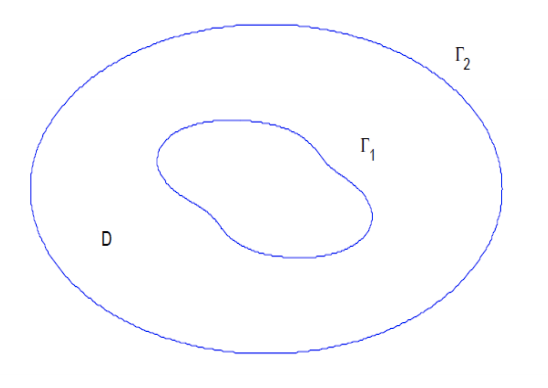
\includegraphics[width=0.55\textwidth]{resources/doubly-connected-region}
		\caption{}
		\label{fig:double-connected-region}
	\end{figure}

	Мішана задача Діріхле-Неймана для рівняння Лапласа полягає в знаходженні такої функції $u(x_1, x_2) \in C^{2}(D)\bigcap  C^{1}(\overline{D})$ що задовольняє

	\begin{enumerate}
		\item
		Рівняння Лапласа: 
		\begin{equation}
			\label{laplace-eq}
			\Delta{u} = 0 \quad \text{в} \quad D
		\end{equation}

		\item
		Граничні умови:
		\begin{equation}
			\label{dirichlet-condition}
			u = f_1 \quad \text{на} \quad \Gamma_1,
		\end{equation}
	
		\begin{equation}
			\label{neumann-condition}
			\pdv{u}{\nu} = f_2 \quad \text{на} \quad \Gamma_2,		
		\end{equation}

	\end{enumerate}
	де $\nu = \nu(x)$ - одиничний вектор зовнішньої нормалі, (\ref{dirichlet-condition}) є умовою Діріхле, а (\ref{neumann-condition}) є умовою Неймана.
	
\newcommand{\boundprob}{(\ref{laplace-eq}) -- (\ref{neumann-condition})} 
	
	
 \newpage
 \thispagestyle{empty}
 \section{Коректність задачі}
 ...
 
 %\subsection{Існування розв'язку}
 \subsection{Єдиність розв'язку задачі}
 \hspace{0.5cm}\theorem{green} Нехай $D$ - область з межею $\partial D \in C^1$ i $\overrightarrow{\nu} -$ одиничний вектор зовнішньої нормалі до межі $\partial D$. Тоді для $u \in C^1(\overline{D})$ і $v \in C^2(\overline{D})$ має місце перша формула Гріна
 $$
 \intl_{D}(u \Delta v+grad u \cdot grad v) d x=\intl_{\partial D} u \frac{\partial v}{\partial \nu} d s
 $$
 i для $u, v \in C^{2}(\overline{D})$ має місце друга формула Гріна
 $$
 \intl_{D}(u \Delta v-v \Delta u) d x=\intl_{\partial D}\left(u \frac{\partial v}{\partial \nu}-v \frac{\partial u}{\partial \nu}\right) d s
 $$
 
 \proof Посилання на Креса.
 
 
 \theorem{single-sol} Нехай $\Gamma_{1}, \Gamma_{2}$ -- гладкі границі, що належать класу $C^1$, обмежують двозв'язну (а може ні?) область $D$. Тоді задача \boundprob \space має на D (може замикання?) не більше одного розв'язку.
 
 \proof Від супротивного. Нехай $\exists u_1, u_2 \in C^{2}(\overline{D}): u_1 \neq u_2 $ -- два різні розв'язки задачі \boundprob. Запишемо цю задачу для функції $u^* = u_1 - u_2$:
 $$
 \Delta u^* = \Delta u_1 - \Delta u_2 = 0
 $$
 $$
 u^* = u_1 - u_2 = f_1 - f_1 = 0 \quad \text{на} \quad \Gamma_1
 $$
 $$
 \frac{\partial u^*}{\partial \nu}
 = \frac{\partial u_1}{\partial \nu} - \frac{\partial u_2}{\partial \nu}
 = f_2 - f_2 = 0 \quad \text{на} \quad \Gamma_2
 $$
 Застосуємо першу формулу Гріна з теореми \ref{green} при $u = v = u^*$:
 $$
 \intl_{D}(\operatorname{grad} u^*)^2 dx
 = \intl_{\partial D} u^* \frac{\partial u^*}{\partial \nu} dS
 - \intl_{D} u^* \Delta u^* dx
 $$
 Тут $\partial D = \Gamma_1 \cup \Gamma_2$. Так як $\Delta u^* = 0 $ (чи ні?) в $D$, $u^*=0$ на $\Gamma_1$ і $\frac{\partial u^*}{\partial \nu} = 0$ на $\Gamma_2$, то отримуємо рівність
 $$
 \intl_{D}(\operatorname{grad} u^*)^2 dx = 0,
 $$
 з якої випливає, що $\frac{\partial u^*}{\partial x_1} = 0$ і $\frac{\partial u^*}{\partial x_2} = 0$ на всій області $D$, тобто $u^* = \operatorname{const}$. Функція $u^*$ неперервна в $\overline{D}$ і $u^*=0$ на $\Gamma_1 \subset \overline{D}$, отже $u^*\equiv0 \Rightarrow u_1\equiv u_2$, що суперечить початковому припущенню. $\blacksquare$
 
 \newpage
 \thispagestyle{empty}
 \section{Зведення до інтегрального рівняння}
 ...
 \subsection{Теорія потенціалів. Потенціал простого шару}


 
 \hspace{0.5cm} Означення гармонічної функції ...
 
 \theorem{fundamental-solution}  Функція
 $$
 \Phi(x, y) := \frac{1}{2\pi} \ln \frac{1}{\abs{x - y}} 
$$
визначена на  $x \neq y,$ $x \in \mathbb{R}$ називається фундаментальним розв'язком рівняння Лапласа. Для фіксованого $y \in \mathbb{R}^2$ вона є гармонічною в $\mathbb{R}^2 \backslash \{y\}$.
 
 
 \defn{single-layer-potential} Нехай функція $\varphi \in C(\partial D),$ тоді
 $$
 u(x):=\intl_{\partial D} \varphi(y) \Phi(x, y) d s(y), \quad x \in \mathbb{R}^{m} \backslash \partial D
 $$
 називають потенціалом простого шару з густиною $\varphi .$
 
 \theorem{potential-on-bound} Нехай $\partial D$ належить класу $C^{2}$ і $\varphi \in C(\partial D) .$ Тоді потенціал простого шару $u$ з густиною $\varphi$ неперервний на $\mathbb{R}^{m} .$ На границі області справджується рівність
 $$
 u(x)=\intl_{\partial D} \varphi(y) \Phi(x, y) d s(y), \quad x \in \partial D
 $$
 де інтеграл існує і розуміється як невласний.
 \proof Кресс
 
 Щось про стрибок ...?
 
 \theorem{potential-partial-derevative} Нехай $\partial D$ належить класу $C^{2} .$ Тоді для потенціалу простого шару $u$ з неперервною густиною $\varphi$ маємо, що
 $$
 \frac{\partial u_{\pm}}{\partial \nu}(x) =
 \intl_{\partial D} \varphi(y) \frac{\partial \Phi(x, y)}{\partial \nu(x)} d s(y) \mp \frac{1}{2} \varphi(x),
 \quad x \in \partial D
 $$
 де
 $$
 \frac{\partial u_{\pm}}{\partial v}(x):=\lim _{h \rightarrow+0} v(x) \cdot \operatorname{grad} u(x \pm h v(x))
 $$
 is to be understood in the sense of uniform convergence on $\partial D$ and where the integral exists as an improper integral.
 
 \subsection{Загальний вигляд розв'язку}
 Потенціал простого шару є гармонічною функцією, тому розв'язок задачі \boundprob \space будемо шукати у вигляді суми потенціалів простого шару
 $$
 u(x) 
 = \intl_{\Gamma_1} \varphi_1(y) \Phi(x, y) d s(y)
 + \intl_{\Gamma_2} \varphi_2(y) \Phi(x, y) d s(y)
 , \quad x \in D
 $$
 з невідомими густинами $\varphi_1 \in C(\Gamma_{1}) $, $\varphi_2 \in C(\Gamma_{2})$.
 
 Враховуючи інтегральне подання розв'язку, крайові умови та властивості потенціалу простого шару, для знаходження невідомих функцій отримаємо таку систему інтегральних рівнянь:
 $$
 \left\{
 \begin{array}{l}
 	\displaystyle
 	  \intl_{\Gamma_{1}} \varphi_1(y) \Phi(x, y) d s(y)
 	+ \intl_{\Gamma_{2}} \varphi_2(y) \Phi(x, y) d s(y)
 	= f_{1}(x), \quad x \in \Gamma_{1} 
 	\\ [0.3cm]
 	\displaystyle
 	  2\intl_{\Gamma_{1}} \varphi_1(y) \frac{\partial \Phi(x, y)}{\partial \nu(x)} d s(y)
 	- \varphi_2(x)
 	+ 2\intl_{\Gamma_{2}} \varphi_2(y) \frac{\partial \Phi(x, y)}{\partial \nu(x)} d s(y)
 	= 2f_{2}(x), \quad x \in \Gamma_{2}
 \end{array}\right.
 $$

 Пояснити про стрибок ...
 (ще раз перевірити на стрибок)
 
 \begin{comment}
 Розв'язок задачі \boundprob \space будемо шукати у вигляді потенціалу простого шару:
 $$
 u(x)=\intl_{\partial D} \varphi(y) \Phi(x, y) d s(y), \quad x \in \mathbb{R}^{m} \backslash \partial D
 $$
 Враховуючи інтегральне подання розв'язку, крайові умови та властивості потенціалу простого шару отримаємо таку систему інтегральних рівнянь:
 $$
 \left\{
 \begin{array}{l}
 \displaystyle \intl_{\Gamma_{1}} \varphi(y) \Phi(x, y) d s(y)=f_{1}(x), \quad x \in \Gamma_{1} 
 \\ [0.3cm]
 \displaystyle \varphi(x) + 2\intl_{\Gamma_{2}} \varphi(y) \frac{\partial \Phi(x, y)}{\partial \nu(x)} d s(y)=2f_{2}(x), \quad x \in \Gamma_{2}
 \end{array}\right.
 $$
 \end{comment}

 \newpage
 \thispagestyle{empty}
 \section{Коректність інтегрального рівняння}
 
 \newpage
 \thispagestyle{empty}
 \section{Параметризація}

 Припустимо, що кривi $\Gamma_{1}$ та $\Gamma_{2}$ заданi в параметричному виглядi:
\begin{equation}
	 \Gamma_{i} := \{ x_{i}(t) = (x_{i1}(t), x_{i2}(t)), \; t \in [ 0, 2\pi ] \} , \quad i = 1, 2
\end{equation}
\indent де $x_{i} : \mathbb{R} \rightarrow \mathbb{R}^2$, $2\pi$ періодична $\forall{t} \; \abs{x'(t)} > 0$

Позначимо $\nu$ - одиничний вектор зовнішньої нормалі до кривої $\Gamma_{i}$, заданий як:
$$
	\nu(x_i(t)) = \left(
	\frac{
		x'_{i2}(t)}{\abs{x'_{i}(t)}
	},
	- \frac{
	x'_{i1}(t)}{\abs{x'_{i}(t)}}
	\right)
$$

Обчислимо похідну по нормалі від фундаментального роз'вязку
$$
\pdv{\Phi(x, y)}{\nu(x)} = -\frac{1}{2\pi} \pdv{\ln(r)}{r}\pdv{r}{\nu(x)}
$$

\indent де $r = \abs{x - y}$, отримаємо

$$
\pdv{\Phi(x, y)}{\nu(x)} = \frac{1}{2\pi} \frac{(y - x) \cdot \nu(x)}{r^2} 
$$

Перейдемо до параметризованої системи. Таким чином використовуючи параметризацію та описані вище перетворення перейдемо до параметризованої системи.
$$
	\left\{
	\begin{array}{l}
		\displaystyle
		\frac{1}{2\pi} \inttwopi \psi_1(\tau) K_{11}(t, \tau) d \tau
		+ \frac{1}{2\pi} \inttwopi  \psi_2(\tau) K_{12}(t, \tau) d \tau
		= g_{1}(t)
		\\ [0.3cm]
		\displaystyle
		- \frac{\psi_2(t)}{\abs{x'_{2}(t))}}
		+ \frac{1}{\pi} \inttwopi \psi_1(\tau) K_{21}(t, \tau) d \tau
		+ \frac{1}{\pi} \inttwopi  \psi_2(\tau) K_{22}(t, \tau) d \tau
		= 2g_{2}(t)
	\end{array}\right.
$$

де $\displaystyle \psi_{i}(t) = \varphi(x_{i}(t)) \cdot \abs{x'_{i}(t)}, \; g_{i} = f_{i}(x_{i}(t)), \;  i  = 1, 2; \; t \in [0, 2\pi]$ \\[0.3cm]
Ядра матимуть вигляд:

$$
	\begin{array}{l}
		\displaystyle
		K_{11}(t, \tau) = \left.
			 \ln{\frac{1}{\abs{x - y}}}
		\right|_{
			{\small \parbox{20mm}{$ x = x_1(t)$ \\[-4pt] $y = x_1 ({\tau})$}}
		} \quad \quad, \quad t \neq \tau
		\\ [0.8cm]
		
		\displaystyle
		K_{12}(t, \tau) = \left.
			\ln{\frac{1}{\abs{x - y}}}
		\right|_{
			{\small \parbox{20mm}{$ x = x_1(t)$ \\[-4pt] $y = x_2 ({\tau})$}}
		} \quad \quad;
		\\ [0.8cm]
		
		\displaystyle
		K_{21}(t, \tau) = \left.
			\frac{(x - y) \cdot \nu(y)}{r^2}
		\right|_{
			{\small \parbox{20mm}{$ x = x_2(t)$ \\[-4pt] $y = x_1 ({\tau})$}}
		};
		\\ [0.8cm]
		
		\displaystyle
		K_{22}(t, \tau) = \left.
			\frac{(x - y) \cdot \nu(y)}{r^2}
		\right|_{
			{\small \parbox{20mm}{$ x = x_2(t)$ \\[-4pt] $y = x_2 ({\tau})$}}
		} 
		, \quad t \neq \tau
	\end{array}
$$

В ядрах $K_{12}$, $K_{21}$ внаслідок параметризації точки $x$ та $y$ знаходяться на різних кривих, з чого випливає що ці ядра неперервні і при інтегруванні в них не виникають особливості.

У випадку $K_{11}$, $K_{22}$ обидві точки знаходяться на одній кривій і тому вони мають, відповідно, логарифмічну і сингулярну особливості при $t = \tau$. 

%Для того щоб їх позбутись, необхідно знайти границі цих ядер при $t \rightarrow \tau$ і використати границю замість ядра для випадків, коли $t = \tau$.

\begin{comment}
K_{22}(t, \tau) = \abs{x'_{2}(\tau)} \left\{
\frac{1}{2} \ln{\frac{1}{\abs{x_2(t) - x_2(\tau)}^2} } \pm \frac{1}{2} \ln{ \left( \frac{4}{e} \sin^2{\frac{t - \tau}{2}} \right) }
\right\}
= - \frac{1}{2} 
\end{comment}

Для  виділення логарифмічної особливості виконаємо наступні перетворення з $K_{11}$
$$
\begin{aligned}
	K_{11}(t, \tau) 
	&=
	\frac{1}{2} \ln \frac{1}{\left|x_{1}(t)-x_{1}(\tau)\right|^{2}} \pm \frac{1}{2} \ln \left(\frac{4}{e} \sin ^{2} \frac{t-\tau}{2}\right)=\\
	&=
	-\frac{1}{2} \ln \left(\frac{4}{e} \sin ^{2} \frac{t-\tau}{2}\right)+\frac{1}{2} \ln \frac{\frac{4}{e} \sin ^{2} \frac{t-\tau}{2}}{\left|x_{1}(t)-x_{1}(\tau)\right|^{2}}
\end{aligned}
$$

Отже, ядро $K_{11}$ можна записати у вигляді:
%де ядра ${K_{11}}^{(1)}$  та  ${K_{11}}^{(2)}$ мають такий вигляд:


$$
	\displaystyle
	K_{11}(t, \tau) = {K_{11}}^{(1)} \ln \left(\frac{4}{e} \sin ^{2}  \frac{t-\tau}{2}\right)+{K_{11}}^{(2)}(t, \tau) \\
$$

де ядра ${K_{11}}^{(1)}$ і ${K_{11}}^{(2)}$ матимуть вигляд:

$$
	\displaystyle
	{K_{11}}^{(1)}(t, \tau) =-\frac{1}{2};
	\displaystyle
	\quad \text{та} \quad
	\displaystyle
	{K_{11}}^{(2)}(t, \tau) =\frac{1}{2} \ln{\frac{\frac{4}{e} \sin ^{2} \frac{t-\tau}{2}}{\left|x_{1}(t)-x_{1}(\tau)\right|^{2}}}, \quad t \neq \tau;
$$

Для того щоб довизначити ${K_{11}}^{(2)}$, знайдему границю за правилом Лопіталя
$$
\lim _{\tau \rightarrow t} K_{11}{ }^{(2)}(t, \tau) = \lim _{\tau \rightarrow t} \ln \frac{\frac{4}{e} \sin ^{2} \frac{t-\tau}{2}}{\left|x_{1}(t)-x_{1}(\tau)\right|^{2}}=\ln \frac{\frac{4}{e} \frac{(t-\tau)^{2}}{4}}{\left|x_{1}^{\prime}(t)\right|^{2}(t-\tau)^{2}}=\ln \frac{1}{e\left|x_{1}^{\prime}(t)\right|^{2}}
$$
В результаті отримаємо:
$$
{K_{11}}^{(2)}(t, \tau) =
\left\{
\begin{array}{l}
	\displaystyle
	\frac{1}{2} \ln{\frac{\frac{4}{e} \sin ^{2} \frac{t-\tau}{2}}{\left|x_{1}(t)-x_{1}(\tau)\right|^{2}}}
	,\quad t \neq \tau
	\\ [1cm]
	
	\displaystyle
	\ln \frac{1}{e\left|x_{1}^{\prime}(t)\right|^{2}}
	,\quad  \quad  \quad \quad  \quad t = \tau
\end{array}
\right.
$$
Виділимо сингулярну особливість ядра $K_{22}$. Знайдемо границю при $\tau \rightarrow t$

\begin{comment}
 $$
 K_{11}(t, \tau) = 
 \left\{
 \begin{array}{l}
 	\displaystyle
	K_{11}(t, \tau) = \left.
	\ln{\frac{1}{\abs{x - y}}}
	\right|_{
		\small \parbox{20mm}{$ x = x_1(t)$ \\[-4pt] $y = x_1 ({\tau})$}
	}, \quad t \neq \tau \\
 	[1cm]

	\displaystyle

	, \quad t = \tau
 \end{array}
 \right.
 $$
\end{comment}

$$
\lim_{\tau \rightarrow t } \pdv{\Phi(x_{2}(t), x_{2}(\tau))}{\nu(t)} =
\frac{ x''_{21}(t) x'_{22}(t) - x''_{22}(t) x'_{21}(t)}{2 \abs{x'_{2}(t)}^2}
$$

Отримаємо наступне параметризованне подання ядра:
 $$
 K_{22}(t, \tau) = 
 \left\{
 \begin{array}{l}
	\displaystyle
	\frac{ x'_{22}(t) (x_{21}(t) - x_{21}(\tau)) - x'_{21}(\tau) (x_{22}(t) - x_{22}(\tau))  }{\abs{x_1(t) - x_1(\tau)}} 
	,\quad t \neq \tau
	\\ [1cm]
	
	\displaystyle
	\frac{ x''_{21}(t) x'_{22}(t) - x''_{22}(t) x'_{21}(t)}{2 \abs{x'_{2}(t)}^2}
	,\quad \quad \quad \quad \quad \quad \quad \quad \quad \quad \quad  t = \tau
	\\ [1cm]	
 \end{array}
 \right.
 $$
  
Отже, система буде мати вигляд
 $$
 \left\{
 \begin{array}{l}
 	\displaystyle
 	\inttwopi \psi_1(\tau) \left\{ {K_{11}}^{(1)} (t, \tau) \ln{\left( \frac{4}{e} \sin^{2}{\frac{t - \tau}{2}} \right) } + {K_{11}}^{(2)} (t, \tau) \right\} d \tau +
 	\\[0.3cm] \qquad \qquad \qquad \qquad \qquad \qquad \qquad \quad
 	\displaystyle
 	+ \inttwopi \psi_2(\tau) K_{12}(t, \tau) d \tau
 	= 2\pi g_{1}(t)
 	\\ [0.3cm]
 	
 	\displaystyle
 	- \pi\frac{\psi_2(t)}{\abs{x'_{2}(t))}}
 	+ \inttwopi \psi_1(\tau) K_{21}(t, \tau) d \tau
 	+ \inttwopi \psi_2(\tau) K_{22}(t, \tau) d \tau
 	= 2\pi g_{2}(t)
 \end{array}\right.
 $$
 
 Використовуючи параметризацію ref можемо записати наближенний розв'язок мішаної задачі ref в параметризованому вигляді:
 $$
 u(x)=\frac{1}{2 \pi} \int_{0}^{2 \pi} \psi_{1}(\tau) K_{1}(x, \tau) d \tau+\frac{1}{2 \pi} \int_{0}^{2 \pi} \psi_{2}(\tau) K_{2}(x, \tau) d \tau, \quad x \in D
 $$
 де відповідні ядра $K_{1}$ і $K_{2}$ мають вигляд:
 $$
  	K_{1}(x, \tau)=\ln \frac{1}{\left|x-x_{1}(\tau)\right|}
  	\quad \text{та} \quad 
 	K_{2}(x, \tau)=\ln \frac{1}{\left|x-x_{2}(\tau)\right|}
 $$
 
 \newpage
 \thispagestyle{empty}
 \section{Чисельне розв'язування}
 
 \subsection{Метод колокації}
 \hspace{0.7cm}...
 
 ...
 
 ...
 
 Шукані функції подамо у вигляді суми ... (сказати щось про n):
 $$
 \tilde{\psi_k}(x)=\sum_{j=1}^{n} c^{(k)}_{j} \gamma^{(k)}_{j}(x), \quad k = 1,2
 $$
 Підставивши їх у систему оримаємо:
 $$
 \left\{
 \begin{array}{l}
 	\displaystyle
 	  \sum_{j=1}^{n} c^{(1)}_{j} \inttwopi \gamma^{(1)}_{j}(\tau) K_{11}(t, \tau) d \tau
 	+ \sum_{j=1}^{n} c^{(2)}_{j} \inttwopi \gamma^{(2)}_{j}(\tau) K_{12}(t, \tau) d \tau
 	= 2\pi g_{1}(t)
 	\\ [0.3cm]
 	
 	\displaystyle
 	  \sum_{j=1}^{n} c^{(1)}_{j} \inttwopi \gamma^{(1)}_{j}(\tau) K_{21}(t, \tau) d \tau
 	\\ [0.3cm]
 	
 	\displaystyle
 	\qquad \qquad \quad
 	+ \sum_{j=1}^{n} c^{(2)}_{j} \left\{
 	    - \pi \frac{\gamma^{(2)}_{j}(t)}{\abs{x'_{2}(t))}}
 	    + \inttwopi \gamma^{(2)}_{j}(\tau) K_{22}(t, \tau) d \tau
 	  \right\}
 	= 2\pi g_{2}(t)
 \end{array}\right.
 $$
 Цю систему необхідно протабулювати n разів по змінній t, щоб знайти відповідні значення векторів $c^{(1)}$ і $c^{(1)}$.
 Запишемо отриману систему у зручному матричному вигляді
 $$
 Ac=g
 $$
 де
 $$
 A =
 \begin{pmatrix}
	 \begin{matrix}
	 	G^{(1)}_{11} & \dots  & G^{(1)}_{1n} \\
	 	\vdots 		 & \ddots & \\
	 	G^{(1)}_{n1} & 		  & G^{(1)}_{nn} \\
	 \end{matrix} &
	 \begin{matrix}
	 	G^{(2)}_{11} & \dots  & G^{(2)}_{1n} \\
	 	\vdots 		 & \ddots & \\
	 	G^{(2)}_{n1} & 		  & G^{(2)}_{nn} \\
	 \end{matrix} \\[1cm]
	 \begin{matrix}
		G^{(3)}_{11} & \dots  & G^{(3)}_{1n} \\
		\vdots 		 & \ddots & \\
		G^{(3)}_{n1} & 		  & G^{(3)}_{nn} \\
	 \end{matrix} &
	 \begin{matrix}
		G^{(4)}_{11} & \dots  & G^{(4)}_{1n} \\
		\vdots 		 & \ddots & \\
		G^{(4)}_{n1} & 		  & G^{(4)}_{nn} \\
	 \end{matrix} \\
 \end{pmatrix}
 c = 
 \begin{pmatrix}
	c^{(1)}_1\\
	\vdots\\
	c^{(1)}_n\\
	c^{(2)}_1\\
	\vdots\\
	c^{(2)}_n\\
 \end{pmatrix}
 g = 
 \begin{pmatrix}
	2\pi g_1(x_1)\\
	\vdots\\
	2\pi g_1(x_n)\\
	2\pi g_2(x_1)\\
	\vdots\\
	2\pi g_2(x_n)\\
 \end{pmatrix}
 $$
 де
 $$
 \begin{matrix}
	G^{(1)}_{ji} = \inttwopi \gamma^{(1)}_{j}(\tau) K_{11}(t_i, \tau) d \tau & \hspace{-1.7cm}
	G^{(2)}_{ji} = \inttwopi \gamma^{(2)}_{j}(\tau) K_{12}(t_i, \tau) d \tau \\[1cm]
	G^{(3)}_{ji} = \inttwopi \gamma^{(1)}_{j}(\tau) K_{21}(t_i, \tau) d \tau & \hspace{1cm}
	G^{(4)}_{ji} = -\pi\frac{\gamma^{(2)}_{j}(t_i)}{\abs{x'_{2}(t_i))}}
				 + \inttwopi \gamma^{(2)}_{j}(\tau) K_{22}(t_i, \tau) d \tau \\
 \end{matrix}
 $$
 
 \subsection{Похибка}
 
 \newpage
 \thispagestyle{empty}
 \section{Якийсь приклад}
 
  \newpage
%%%%%%%%%%%%%%%%%%%%%%%%%%%%%%%%%%%%%%%%%%%%%%%%%%%%%%%%%%%%%%%%%%	
\nocite{kress2012linear}
\printbibliography[title={Бібліографія}]
%%%%%%%%%%%%%%%%%%%%%%%%%%%%%%%%%%%%%%%%%%%%%%%%%%%%%%%%%%%%%%%%%%

\end{document}
 
 